\documentclass[tikz,border=5pt]{standalone}
\usepackage{pgfplots}
\usetikzlibrary{calc}
\pgfplotsset{compat=1.17}

\begin{document}
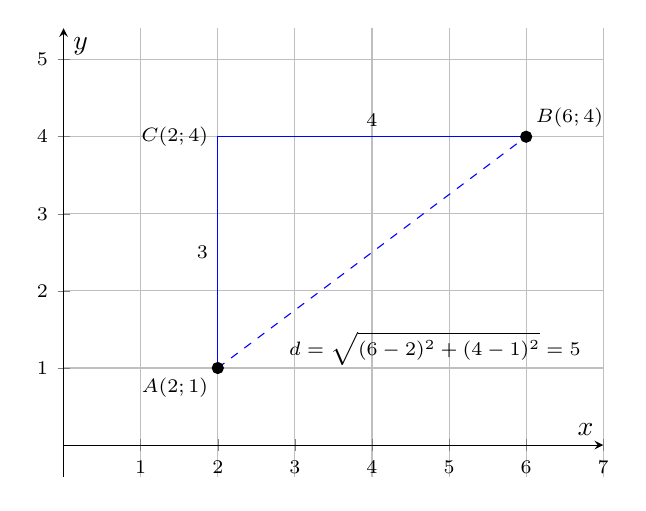
\begin{tikzpicture}
\begin{axis}[
    label style={font=\scriptsize},
    tick label style={font=\scriptsize},
    axis lines=middle,
    axis equal,
    grid=major,
    xmin=0, xmax=7,
    ymin=0, ymax=5,
    xtick={0,1,2,3,4,5,6,7},
    ytick={0,1,2,3,4,5},
    xlabel={$x$},
    ylabel={$y$}
]

% Define points A and B
\coordinate (A) at (2,1);
\coordinate (B) at (6,4);

% Define point C to complete the right angle
\coordinate (C) at (2,4);

% Plot points A and B
\addplot[only marks, mark=*] coordinates {(2,1) (6,4)};

% Draw the right triangle
\draw[blue] (A) -- (C) -- (B);

% Draw the hypotenuse (distance line)
\draw[blue, dashed] (A) -- (B);

% Labels
\node[below left] at (A) {\scriptsize$A(2;1)$};
\node[above right] at (B) {\scriptsize$B(6;4)$};
\node[left]       at (C) {\scriptsize$C(2;4)$};

% Horizontal and vertical distances
\node[left]  at ($(A)!0.5!(C)$) {\scriptsize$3$};
\node[above] at ($(C)!0.5!(B)$) {\scriptsize$4$};

% Label the distance formula
\node[sloped, below right] at ($(A)!0.2!(B)$) 
    {\scriptsize$d = \sqrt{(6-2)^2 + (4-1)^2} = 5$};

\end{axis}
\end{tikzpicture}\end{document}
